\documentclass[table]{beamer}
\usepackage[T1]{fontenc}
\usepackage{mdwlist}
\usepackage{multirow}
\usepackage{graphicx}
\usepackage{verbatim} % For using /begin{comment}; /end{comment}

%\usepackage{selinput} % ?
%Loading a font package, uncomment one of the following lines to see changes
%\usepackage{libertine}
%\usefonttheme{default}
%\usefonttheme{professionalfonts}

%\setbeamerfont{frametitle}{series=\bfseries} % Frame titles should be bold

\usepackage{lmodern}

% Bright colors
\definecolor{oj}{rgb}{1.0,0.65,0.0}
\definecolor{cblue}{rgb}{0.39,0.58,0.93}
\definecolor{amethyst}{rgb}{0.6, 0.4, 0.8}

% Pale colors
\definecolor{lightgrey}{rgb}{0.75, 0.75, 0.80}
\definecolor{tangerine}{rgb}{1.0, 0.6, 0.4}
\definecolor{arylyellow}{rgb}{0.91, 0.84, 0.42}
\definecolor{gsa}{rgb}{0.66, 0.89, 0.63}
\definecolor{aqua}{rgb}{0.5, 1.0, 0.83}
\definecolor{bblue}{rgb}{0.67, 0.9, 0.93}

\setbeamercolor{normal text}{bg=black, fg=lightgrey}
\setbeamercolor{title}{fg=arylyellow}
\setbeamercolor{frametitle}{fg=tangerine}
\setbeamercolor{framesubtitle}{fg=gsa}
\setbeamercolor{block title}{fg=aqua}
\setbeamercolor{itemize item}{fg=amethyst} % all frames will have red bullets
\setbeamercolor{enumerate item}{fg=amethyst} % all frames will have red bullets
%\setbeamercolor{block title}{fg=green}


\setbeamertemplate{itemize items}[circle]
\title{\textbf{Coronal Seismology}}
\subtitle{\textbf{ASTR 598}}
\date{\textbf{Spring 2016}}
\author{\textbf{Laurel Farris}}

\begin{document}

{\usebackgroundtemplate{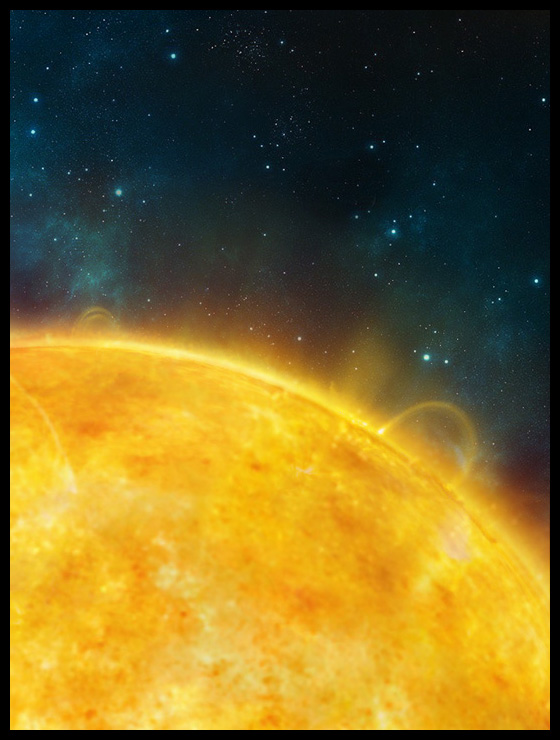
\includegraphics[width=\paperwidth]
    {awesome.jpg}}
\begin{frame}
    \titlepage{}
\end{frame}}%-------------------------------------------------------------%
\begin{frame}{Magnetohydrodynamics (MHD)}{Theory}
    %[Relationship between size and decay time].
    \begin{columns}
        \column{0.5\textwidth}
        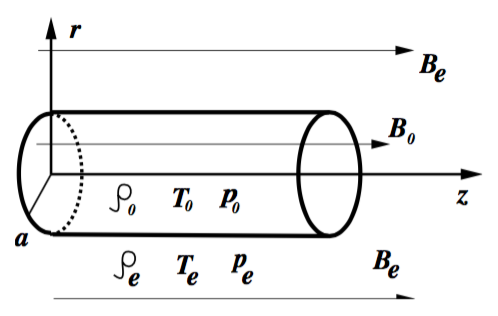
\includegraphics[width=\textwidth]{cylinder.png}
        \column{0.5\textwidth}
        \begin{itemize}
            \item Straight flux tube in uniform magnetic field.
            \item $ \xi(x) = \xi(r)e^{i(kz+m{\phi})} $
            \item Characteristic speeds are determined by the
                environment
        \end{itemize}
    Types of waves/oscillations:
    \begin{itemize}
        \item Alfv\'en: $V_A = \frac{B}{\mu_0\rho}$
        \item Magnetoacoustic: $C_s = \sqrt{\frac{\gamma P}{\rho}}$
            \begin{itemize}
                \item Fast $C_{A_0} < C_{fast} < C_{A_e} $
                \item Slow $C_{T_0} < C_{slow} < C_{s_0} $
            \end{itemize}
    \end{itemize}
    \end{columns}
\end{frame}%-------------------------------------------------------------%
\begin{frame}{Coronal seismology}{Technique and motivation}
    Problem: properties of the corona, such as magnetic field strength,
    densities, and Alfv\'en velocities, are difficult to measure.

    Solution: coronal seismology.
    \begin{itemize}
        \item Observe disturbances in the corona:
            \begin{itemize}
                \item Period
                \item Velocity
                \item Timescales
            \end{itemize}
        \item Compare observed quantities to MHD theory to identify the
            type of wave or mode.
        \item Insert observed properties into appropriate equations to
            derive coronal parameters.
    \end{itemize}
    Current questions:
    \begin{itemize}
        \item How are these disturbances initiated?
        \item How are they damped, and what determines the timescales?
    \end{itemize}
    Motivation:
    \begin{itemize}
        \item Coronal heating problem
        \item Constraining flare/CME environment
    \end{itemize}
\end{frame}%-------------------------------------------------------------%
\begin{frame}{Coronal seismology}
    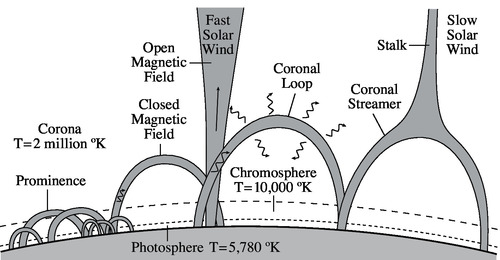
\includegraphics[width=\textwidth]{loop_diagram.jpg}
\end{frame}%-------------------------------------------------------------%
\begin{frame}{Dispersion diagram}
    \begin{figure}
        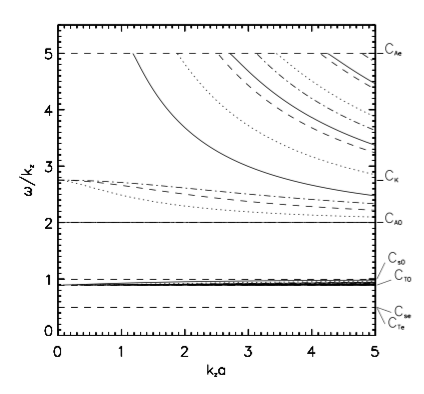
\includegraphics[width=3in]{disp_diagram.png}
    \end{figure}
\end{frame}%-------------------------------------------------------------%
\begin{frame}{MHD modes}{Oscillations vs.\ waves}
    (Or magnetoacoustic vs.\ Alfv\'en.)
    (Or fast vs.\ slow.)
    [insert characteristic speeds, periods, how observed, etc.\ here].
    \begin{itemize}
        \item Fast standing oscillations
            \begin{itemize}
                \item Kink
                \item Sausage
            \end{itemize}
        \item Slow standing oscillations
            \begin{itemize}
                \item Acoustic
            \end{itemize}
        \item Propagating slow waves
            \begin{itemize}
                \item Acoustic
            \end{itemize}
        \item Propagating fast waves
            \begin{itemize}
                \item Moreton
                \item EIT waves
            \end{itemize}
        \item Torsional modes (aka.\ Alfv\'en waves)
    \end{itemize}
\end{frame}%-------------------------------------------------------------%
\begin{frame}{Fast standing oscillations}{Kinks vs.\ Sausages}
%\begin{center}
\begin{columns}
        \column{0.6\textwidth}
        \framebox{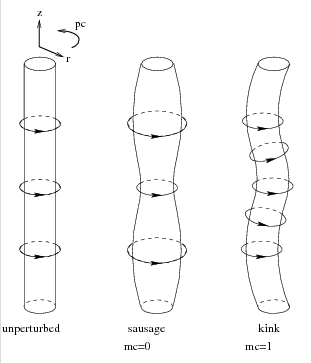
\includegraphics[width=2.5in]{kink_saus.png}}
    %\par{\tiny image credit:\\
    %$https://inspirehep.net/record/1088737/files/figures_instab_locations.png$}
    %\end{center}
        \column{0.4\textwidth}
    \begin{block}{Kink}
        \begin{itemize}
            \item loop spatial displacement
            \item Asymmetric
            \item No intensity change
            \item $k\sigma \ll 1$, or $\sigma\ll\lambda$
        \end{itemize}
    \end{block}
    \begin{block}{Sausage}
        \begin{itemize}
            \item No loop spatial displacement
            \item Symmetric
            \item Intensity change\\ $\rightarrow$ density change
            \item $\lambda\sim\sigma$
            \item long-wavelength limit
        \end{itemize}
    \end{block}
\end{columns}
\end{frame}%-------------------------------------------------------------%

%========================================================================%
\begin{comment}
\begin{frame}{Kink modes}{general characteristics}
    \begin{itemize}
        \item $c_k=\sqrt{\frac{\rho_oV_{Ao}^2 + \rho_cV_{Ac}^2}
            {\rho_o + \rho_c}}
            \approx V_A\sqrt{\frac{2}{1+\frac{\rho_e}{\rho_o}}} $
            in the low-$\beta$ plasma.
        \item $v_{ph} = \frac{\omega}{k} \approx C_k \gtrsim V_A $
        \item Period $P=\frac{2l}{V_A}\sqrt{\frac{1+\rho_e/\rho_o}{2}}$
            where $\lambda=2l$ ($l$ is the loop length).
            Typically, $l \approx 60-600$ Mm in the corona.
        \item ``current pinch'' instability
        \item Important observation from which magnetic field strength
            can be derived.
    \end{itemize}
\end{frame}%-------------------------------------------------------------%
\begin{frame}{Research Goals}
    [insert full disk here, as background or side image]
    \begin{itemize}
        \item Learn what the field is doing (review articles).
        \item Global contribution to topic --- variety of authors,
            work done within the last five years or so.
        \item Fit research into the ``big picture''
    \end{itemize}
\end{frame}%-------------------------------------------------------------%
\begin{frame}{Kink modes}
{Coronal loop oscillations observed with the
\emph{Transition Region And Coronal Explorer (TRACE)}}
    \begin{itemize}
        \item Not just a single, global mode.
        \item Gaussian vs.\ exponential
        \item Plasma motions around footpoints of coronal loops
    \end{itemize}
\end{frame}%-------------------------------------------------------------%
\begin{frame}{Kink modes}{``Excitation and damping of broadband kink waves
    in the solar corona''}
    Footpoint-driven, \emph{propagating} kink waves (which are
    temporally and spatially ubiquitous in the corona).
    Both standing and propagating kink waves are rapidly damped.
\end{frame}%-------------------------------------------------------------%
\begin{frame}{Sausage modes}{The basics}
    Trapped fast modes supported by thick, dense loops because of the
    cutoff wavenumber (pfw\_2). Observe spatially resolved radio
    (see sources in pfw\_2).
\end{frame}%-------------------------------------------------------------%
\begin{frame}{Sausage modes}{Observations of sausage modes in magnetic pores}
\end{frame}%-------------------------------------------------------------%
\begin{frame}{Sausage modes}{Sausage waves in transversely nonuniform
    monolithic coronal tubes}
\end{frame}%-------------------------------------------------------------%
\begin{frame}{Standing acoustic oscillations}
    [Insert movie here?]
    Characteristics:
    \begin{itemize}
        \item Pressure forces in opposition
        \item Period = 7--31 minutes (20 minutes from another source)
        \item Decay times = 5.7--36.8 minutes
        \item Peak velocity = 200 km/sec
    \end{itemize}
\end{frame}%-------------------------------------------------------------%
\begin{frame}{Standing oscillations vs.\ propagating waves}
    \begin{itemize}
        \item In loops, propagating waves damp before
            reaching opposite footpoint.
        \item Velocity and intensity are 90$^{\circ}$ out of phase
            for standing oscillations, and are in phase for propagating
            acoustic waves.
        \item Frequencies less than the cutoff are standing oscillations,
            waves with frequency greater than the cutoff propagate into
            the chromosphere.
        \item no loop shape change or displacement
        \item near footpoints.
    \end{itemize}
\end{frame}%-------------------------------------------------------------%
\begin{frame}{Propagating acoustic waves}{Slow}
    \begin{itemize}
        \item $v_{ph}<150$ km s$^{-1}$ $\rightarrow$ slow
        \item longitudinal, compressive, anisotropic
        \item Parallel to $\vec{B}$, perturbation of $\vec{B}$ is negligible.
        \item Generated impulsively at one end of a footpoint.
        \item Only penetrate $\sim$ 10\% into loop before
            damped by thermal conduction
        \item weak dispersion in coronal conditions ($V_{A} \gg c_{s}$)
        \item 3 phases: periodic, QP, decay
        \item period = 3, 5, 10 minutes? Or 2--22 seconds? (see kink\_1),
        \item velocity: 50--200 km s$^{-1}$
        \item $c_{T} = \sqrt{\frac{c_{s}^2v_{A}^2}{c_{s}^2 + v_{A}^2}} $
            propagate sub-sonically at $c_{T}$, which is less than $c_{s}$
        \item ``large'' amplitude, max in top of chromosphere
        \item Observed using spectroscopy (intensity variations in
            EUV emission  and Doppler shifts)
    \end{itemize}
\end{frame}%-------------------------------------------------------------%
\begin{frame}{pac\_1}
\end{frame}%-------------------------------------------------------------%
\begin{frame}{pac\_2}
\end{frame}%-------------------------------------------------------------%
\begin{frame}{Propagating acoustic waves}{Fast}
    \begin{itemize}
        \item $v_{ph}>150$ km s$^{-1}$ $\rightarrow$ fast
            (\emph{or} transverse standing waves).
        \item Quasi-isotropic
        \item Driven by magnetic forces + plasma pressure forces
        \item Compressive (magnetic sound wave)
        \item Speed: $c_{F} = \sqrt{c_{s}^2 + v_{A}^2} $
        \item Moreton waves in the chromosphere
        \item Fast EUV waves in the corona
    \end{itemize}
\end{frame}%-------------------------------------------------------------%
\begin{frame}{``FIRST SIMULTANEOUS OBSERVATION OF AN H$\alpha$
    MORETON WAVE, EUV WAVE, AND FILAMENT/PROMINANCE OSCILLATIONS''}
    {Asai, et al. (pfw\_2)}
\end{frame}%-------------------------------------------------------------%
\begin{frame}{pfw\_2}
\end{frame}%-------------------------------------------------------------%
\begin{frame}{Torsional modes}{aka.\ Alfv\'en wave}
    Properties:
    \begin{itemize}
        \item m$=$0 (Axisymmetric, or azimuthally symmetric)
        \item transverse (shear) perturbations
        \item Parallel to $\vec{B}$
        \item Driving force: magnetic tensioin
        \item incompressible
        \item velocity: $v_{A} = \frac{B}{\mu_{o}\rho}$;
            $\sim$ 1000 km s$^{-1}$ in the corona
    \end{itemize}
    How to observe:
    \begin{itemize}
        \item Only get Doppler shifts from \emph{long}-period waves
            ($>$ a few minutes).
        \item Measure additional (i.e.\ non-thermal) broadening
            of coronal emission lines; indirect way to observe short-period waves.
        \item Spatial variation in Doppler shift for long periods.
            Gyrosynchrotron emission in radio regime.
    \end{itemize}
    Effects of twisting:
    \begin{itemize}
        \item Coupling of various MHD modes
    \end{itemize}
\end{frame}%-------------------------------------------------------------%
\begin{frame}{tor\_1}
\end{frame}%-------------------------------------------------------------%
\begin{frame}{tor\_2}
\end{frame}%-------------------------------------------------------------%
\end{comment}
%========================================================================%
\begin{frame}{Important Properties}
    \begin{center}
        \begin{tabular}{c|c|c|c|}
            \cline{2-4} & {\textbf{period}} & {\textbf{wavelength}} &
                {\textbf{velocity}}\\
            \hline \multicolumn{0}{|c|}{kink osc} & value & value & value\\
            \hline \multicolumn{0}{|c|}{sausage osc} & value & value & value\\
            \hline \multicolumn{0}{|c|}{acoustic osc} & value & value & value\\
            \hline \multicolumn{0}{|c|}{acoustic waves} & value & value & value\\
            \hline \multicolumn{0}{|c|}{fast waves} & value & value & value\\
            \hline \multicolumn{0}{|c|}{torsional modes} & 10 m & value &
                1000 km s$^{-1}$\\
            \hline
        \end{tabular}
    \end{center}
\end{frame}%-------------------------------------------------------------%
%========================================================================%
\begin{comment}
\begin{frame}{Example Table}
\begin{center}
   \begin{tabular}{cc|c|c|}
% row 1
   \cline{3-4} & & \multicolumn{2}{|c|}{Condition (Gold standard)}\\
% row 2
   \cline{3-4} & & True & False \\
   \hline
% row 3 (and 4) - multirow
   \multicolumn{1}{|c|} % add in vertical lines
   {\multirow{2}{*}{Test outcome}}& % Text covers rows 3 and 4
 % row 3
   \multicolumn{1}{|c|}{Positive} %
     & True Positive \cellcolor{green} & False Positive\cellcolor{red}\\
 % row 4
   \cline{2-4} \multicolumn{1}{|c|}{}
     & \multicolumn{1}{|c|}{Negative}
     & False Negative\cellcolor{red} & True Negative \cellcolor{green}\\
    \hline
    \end{tabular}
\end{center}
\end{frame}%-------------------------------------------------------------%
\begin{frame}{Example of Two Column Output}
    \begin{columns}[c]
        \column{1.5in}
            Practical \TeX\ 2005\\
            Practical \TeX\ 2005\\
            Practical \TeX\ 2005
        \column{1.5in}
            % put nice little frame around graphic
            \framebox{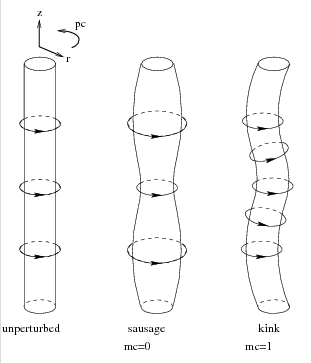
\includegraphics[width=1.5in]{kink_saus.png}}
    \end{columns}
\end{frame}%-------------------------------------------------------------%
\begin{frame}{Research}
    \includegraphics[width=\paperwidth]{figures/full.png}
\end{frame}%-------------------------------------------------------------%
\begin{frame}{Research}
    \includegraphics[width=\paperwidth]{figures/bp1.png}
\end{frame}%-------------------------------------------------------------%
\begin{frame}{Research}
    \includegraphics[width=5in]{figures/bp1_image.png}
\end{frame}%-------------------------------------------------------------%
%========================================================================%
\begin{frame}{Research}{[put full disk at beginning]}
    \framebox{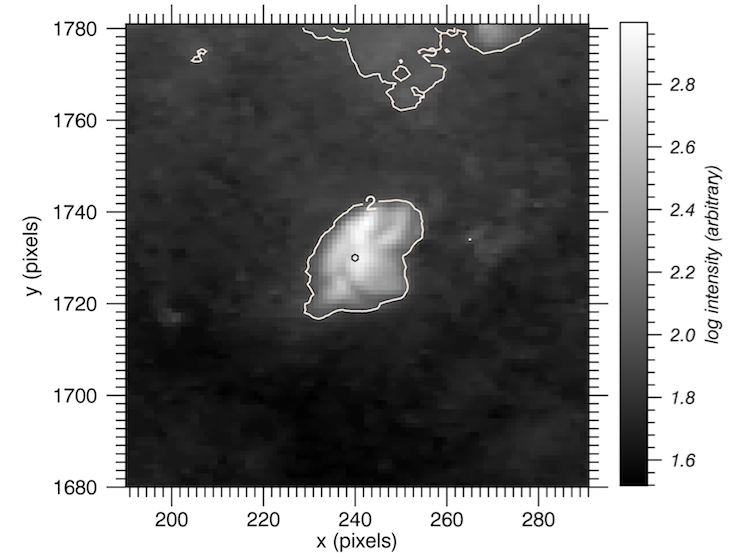
\includegraphics[width=0.8\paperwidth]{figures/bp1_contour.png}}
\end{frame}%-------------------------------------------------------------%
\begin{frame}{Research}
    \hspace{-0.08\paperwidth}
    \framebox{\includegraphics[width=0.9\paperwidth]{figures/bp1_cool2.png}}
\end{frame}%-------------------------------------------------------------%
\end{comment}

\end{document}
